\chapter{Results}
In order to visually demonstrate the encryption, visualisations of the ciphertext polynomial $c_0$ (refer to \autoref{sec:ckks}) were generated using a CRT decomposition of the RNS representation of $c_0$.
Each pixel corresponds to a coefficient $a \in \Z / q\Z$ scaled down by the modulus $q$ to obtain a brightness value between $0$ and $1$.

\begin{figure}[H]
  \centering
  % 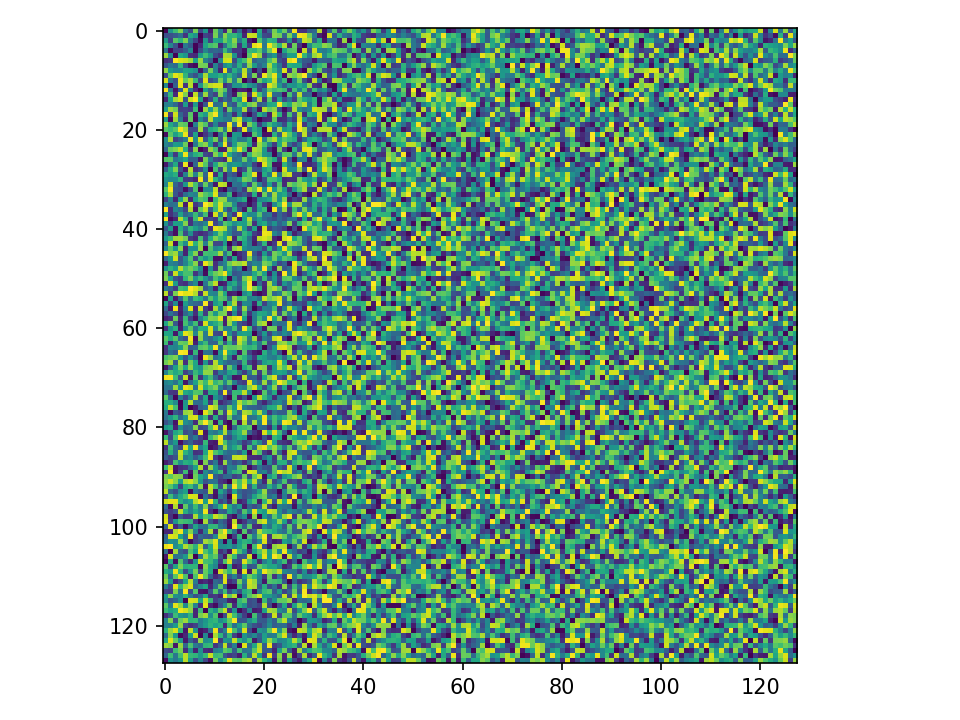
\includegraphics[width=\linewidth]{figures/ciphertext-visualisation.png}
  \pgfplotsset{/pgfplots/group/.cd,vertical sep=0.3cm,horizontal sep=0.3cm}
  % This file was created with tikzplotlib v0.10.1.
\def\ciphertextimagesize{0.25\linewidth}
\begin{tikzpicture}
  \definecolor{darkgray176}{RGB}{176,176,176}
  \begin{groupplot}[group style={group size=5 by 2}]
    \nextgroupplot[
      height=\ciphertextimagesize,
      hide x axis,
      hide y axis,
      tick align=outside,
      tick pos=left,
      width=\ciphertextimagesize,
      x grid style={darkgray176},
      xmin=-0.5, xmax=27.5,
      xtick style={color=black},
      y dir=reverse,
      y grid style={darkgray176},
      ymin=-0.5, ymax=27.5,
      ytick style={color=black}
    ]
    \addplot graphics [includegraphics cmd=\pgfimage,xmin=-0.5, xmax=27.5, ymin=27.5, ymax=-0.5] {figures/generated/ciphertext-visualisation-000.png};

    \nextgroupplot[
      height=\ciphertextimagesize,
      hide x axis,
      hide y axis,
      tick align=outside,
      tick pos=left,
      width=\ciphertextimagesize,
      x grid style={darkgray176},
      xmin=-0.5, xmax=127.5,
      xtick style={color=black},
      y dir=reverse,
      y grid style={darkgray176},
      ymin=-0.5, ymax=127.5,
      ytick style={color=black}
    ]
    \addplot graphics [includegraphics cmd=\pgfimage,xmin=-0.5, xmax=127.5, ymin=127.5, ymax=-0.5] {figures/generated/ciphertext-visualisation-001.png};

    \nextgroupplot[
      height=\ciphertextimagesize,
      hide x axis,
      hide y axis,
      tick align=outside,
      tick pos=left,
      width=\ciphertextimagesize,
      x grid style={darkgray176},
      xmin=-0.5, xmax=27.5,
      xtick style={color=black},
      y dir=reverse,
      y grid style={darkgray176},
      ymin=-0.5, ymax=27.5,
      ytick style={color=black}
    ]
    \addplot graphics [includegraphics cmd=\pgfimage,xmin=-0.5, xmax=27.5, ymin=27.5, ymax=-0.5] {figures/generated/ciphertext-visualisation-002.png};

    \nextgroupplot[
      height=\ciphertextimagesize,
      hide x axis,
      hide y axis,
      tick align=outside,
      tick pos=left,
      width=\ciphertextimagesize,
      x grid style={darkgray176},
      xmin=-0.5, xmax=127.5,
      xtick style={color=black},
      y dir=reverse,
      y grid style={darkgray176},
      ymin=-0.5, ymax=127.5,
      ytick style={color=black}
    ]
    \addplot graphics [includegraphics cmd=\pgfimage,xmin=-0.5, xmax=127.5, ymin=127.5, ymax=-0.5] {figures/generated/ciphertext-visualisation-003.png};

    \nextgroupplot[
      height=\ciphertextimagesize,
      hide x axis,
      hide y axis,
      tick align=outside,
      tick pos=left,
      width=\ciphertextimagesize,
      x grid style={darkgray176},
      xmin=-0.5, xmax=27.5,
      xtick style={color=black},
      y dir=reverse,
      y grid style={darkgray176},
      ymin=-0.5, ymax=27.5,
      ytick style={color=black}
    ]
    \addplot graphics [includegraphics cmd=\pgfimage,xmin=-0.5, xmax=27.5, ymin=27.5, ymax=-0.5] {figures/generated/ciphertext-visualisation-004.png};

    \nextgroupplot[
      height=\ciphertextimagesize,
      hide x axis,
      hide y axis,
      tick align=outside,
      tick pos=left,
      width=\ciphertextimagesize,
      x grid style={darkgray176},
      xmin=-0.5, xmax=127.5,
      xtick style={color=black},
      y dir=reverse,
      y grid style={darkgray176},
      ymin=-0.5, ymax=127.5,
      ytick style={color=black}
    ]
    \addplot graphics [includegraphics cmd=\pgfimage,xmin=-0.5, xmax=127.5, ymin=127.5, ymax=-0.5] {figures/generated/ciphertext-visualisation-005.png};

    \nextgroupplot[
      height=\ciphertextimagesize,
      hide x axis,
      hide y axis,
      tick align=outside,
      tick pos=left,
      width=\ciphertextimagesize,
      x grid style={darkgray176},
      xmin=-0.5, xmax=27.5,
      xtick style={color=black},
      y dir=reverse,
      y grid style={darkgray176},
      ymin=-0.5, ymax=27.5,
      ytick style={color=black}
    ]
    \addplot graphics [includegraphics cmd=\pgfimage,xmin=-0.5, xmax=27.5, ymin=27.5, ymax=-0.5] {figures/generated/ciphertext-visualisation-006.png};

    \nextgroupplot[
      height=\ciphertextimagesize,
      hide x axis,
      hide y axis,
      tick align=outside,
      tick pos=left,
      width=\ciphertextimagesize,
      x grid style={darkgray176},
      xmin=-0.5, xmax=127.5,
      xtick style={color=black},
      y dir=reverse,
      y grid style={darkgray176},
      ymin=-0.5, ymax=127.5,
      ytick style={color=black}
    ]
    \addplot graphics [includegraphics cmd=\pgfimage,xmin=-0.5, xmax=127.5, ymin=127.5, ymax=-0.5] {figures/generated/ciphertext-visualisation-007.png};

    \nextgroupplot[
      height=\ciphertextimagesize,
      hide x axis,
      hide y axis,
      tick align=outside,
      tick pos=left,
      width=\ciphertextimagesize,
      x grid style={darkgray176},
      xmin=-0.5, xmax=27.5,
      xtick style={color=black},
      y dir=reverse,
      y grid style={darkgray176},
      ymin=-0.5, ymax=27.5,
      ytick style={color=black}
    ]
    \addplot graphics [includegraphics cmd=\pgfimage,xmin=-0.5, xmax=27.5, ymin=27.5, ymax=-0.5] {figures/generated/ciphertext-visualisation-008.png};

    \nextgroupplot[
      height=\ciphertextimagesize,
      hide x axis,
      hide y axis,
      tick align=outside,
      tick pos=left,
      width=\ciphertextimagesize,
      x grid style={darkgray176},
      xmin=-0.5, xmax=127.5,
      xtick style={color=black},
      y dir=reverse,
      y grid style={darkgray176},
      ymin=-0.5, ymax=127.5,
      ytick style={color=black}
    ]
    \addplot graphics [includegraphics cmd=\pgfimage,xmin=-0.5, xmax=127.5, ymin=127.5, ymax=-0.5] {figures/generated/ciphertext-visualisation-009.png};
  \end{groupplot}
\end{tikzpicture}

  \caption{Ciphertext Visualisation}
\end{figure}

\section{Methodology}

\section{Accuracy, Precision, Recall}
% Detailliertere Analyse
% https://medium.com/analytics-vidhya/accuracy-precision-and-recall-in-machine-learning-classification-ae84004e86a1
% https://en.wikipedia.org/wiki/Precision_and_recall

\section{Performance Benchmarks}
This chapter includes runtime and communication overhead analysis.

Plain runtime: xxx

\begin{table}[H]
  \centering
  \caption{Performance Benchmarks / Communication Overhead}
  \begin{tabular}{lllll}
    \textbf{Scenario} & \textbf{Parameters} & \textbf{Runtime} / \si{\second} & \textbf{Message Size} / \si{\mega\byte} &   & \textbf{MRE} \\
    BSGS Matmul       & 60,40,...,40,60     &                                 &                                         &                  \\
    BSGS Matmul       & 34,25,...,25,34     &                                 &                                         &                  \\
    Hybrid Matmul     &                     &                                 &                                         &                  \\
    Encrypt           &                     &                                 &                                         &                  \\
    Encrypt Symmetric &                     &                                 &                                         &                  \\
  \end{tabular}
\end{table}
